\documentclass[12 pt]{article}
\usepackage[utf8]{inputenc}
\usepackage{graphicx}
\usepackage{amsmath}
\usepackage[version=4]{mhchem}
\usepackage{siunitx}
\usepackage{longtable,tabularx}
\usepackage{float}
\usepackage[left=1in, right=1in]{geometry}
\usepackage{pdfpages}

\title{MECH6066 HW\#2}
\date{10.05.25}
\author{Slade Brooks \\ M13801712}

\begin{document}
\maketitle

\section*{Problem 1}
\subsection*{(a)}
Yes, this matches my expectations. A quiet room is typically quoted around 25--30 dB, and my air conditioning was
running during the measurements so it makes sense to be slightly high.
\begin{figure}[H]
    \centering
    \includegraphics[width=0.5\linewidth]{figs/hw2figbackground.jpg}
\end{figure} \par

\subsection*{(b)}
At 50\%, the FFT showed 62dB. At 75\%, it showed 65dB. At 100\%, it showed 68dB. I felt like 75\% was not that much
louder, but 100\% felt much louder than 50\%. I think the increase between 50\%--75\% and 75\%-100\% felt like the same
difference.

\subsection*{(c)}
I had measured S1 at 62dB, and set S2 to 61dB. Together, I measured them at 64dB. Since these are uncorrelated sources,
we can sum the intensity. Using an online calculator to convert each to intensity, then summing and getting SIL we
calculate that the measured value should be 64.55dB. This is very close to the 64dB I measured, and a number of setup
issues could cause the slight discrepancy.

\subsection*{(d)}
I ended up with both S1 and S2 measuring 62dB. The fluctuation in the time history could be caused by phasing. Since the
sources are not necessarily in phase, the total measured can fluctuate. In theory, the maximum is two in phase which
would be 68dB and the minimum would be 180deg out of phase which would totally cancel out and measure only the
background level of 41dB. I measured a maximum of roughly 72dB and a minimum of 59dB. I measured a little bit higher
than this, but my background noise was changing a little bit so this may be an increase in background during the
measurement. The two signals clearly never went completely out of phase, as I always heard a tone, which means my
minimum will be higher than the background.

\subsection*{(e)}
The spectrum is pretty close, but not exact. There is a fairly flat band from 1kHz--10kHz, but there are visible peaks
and valleys within that range. The average value appears to be constant. The white noise will not show an exactly flat
response due to the speakers response, and the fact that we have A-weighting applied. It is unlikely to ever be a
perfect flat frequency output.
\begin{figure}[H]
    \centering
    \includegraphics[width=0.5\linewidth]{figs/hw2fig1.jpg}
\end{figure} \par
The SPL at the 125Hz band is roughly 20dBA. This would be 36.2dB unweighted based on the conversion table. This would be
much closer to the value measured at the other frequency bands, and the full unweighted conversion may show a flatter
response for the white noise.
\begin{figure}[H]
    \centering
    \includegraphics[width=0.5\linewidth]{figs/hw2fig2.jpg}
\end{figure} \par
I ended up getting both sources to measure 70dB individually. Together, I measured them at 73dB. The calculated value
for the sum, since they are uncorrelated noise, is the sum of intensities, which would give 73dB. My measurement was
very accurate to the expected value.

\subsection*{(f)}
The white noise is much more comfortable. While it is still loud and you can feel how loud it is, it is much more
pleasant to hear white noise. The single tone is incredibly annoying and it gets stuck in your head even after it ends.
The white noise can reach an unpleasant volume, but it does not stick in your head or bother me as much as a single tone
does. This makes a lot of sense as people typically enjoy white noise, but hearing a constant tone like a buzzing sound
would be super annoying.

\section*{Problem 2}
\subsection*{(a)}
I would select the Teledyne TC4038 for measuring the transducer output. Firstly, we want a hydrophone capable of at
least double the frequency we are interested in. Teledyne only had 2 options that measured over 500kHz. I selected the
TC4038 because while it is rated for less depth and does not have a built-in pre-amp, it is described as a standard
reference hydrophone that is ``traceable to national standards''. It is also described as ideal for near-field
measurements. Overall, it seems perfect for characterization of a transducer. The other option, the TC4035, appears to
be a more applied version of the hyrdophone. It is rated for high depth and has an integrated pre-amp, so it would be
much more useful in a real application. The TC4038 that I selected has a sensitivity of -228 dB re. 1Vrms/$\mu$Pa, which
is equal to $3.981\cdot10^{-6}$ V/Pa.

\subsection*{(b)}
\begin{align*}
    V_{out}=S\cdot p_{hyd}=3.981\cdot10^{-6}\left(55000+j389000\right)=0.219+j1.549\text{ V} \\
    |V_{out}|=\sqrt{0.219^2 + 1.549^2}=\fbox{$1.564\text{ V}=|V_{out}|$} \\
    \phi_{out}=\arctan\left(1.549/0.219\right)=\fbox{$81.95^{\circ}=\phi_{out}$}
\end{align*}

\subsection*{(c)}
\begin{align*}
    p_{rms}=|p_{hyd}|/\sqrt{2}=\left(\sqrt{55^2+389^2}\right)/\sqrt{2}=277.8\text{ kPa}=277800\text{ Pa}
\end{align*}
\begin{align*}
    p_{SPL}=20\log_{10}\left(\frac{277800}{1\cdot10^{-6}}\right)=\fbox{$228.9\text{ dB}=p_{SPL}$}
\end{align*}

\subsection*{(d)}
\begin{align*}
    S=\frac{\sqrt{55000^2+389000^2}}{10}=\fbox{$39287\text{ Pa/V}=S_{trans}$}
\end{align*}

\subsection*{(e)}
I do not believe enough information is given to calculate the speed of sound. Assuming the phase shift is from
propagation time gives a speed of sound of over 100000 m/s, which is clearly wrong for water. I also attempted to solve
for k in the $V_{out}$ equation, but without knowing the measured voltage at some time, there is not enough information.
I also attempted to solve using SIL, but that requires assuming a reference intensity for water based on a specific
speed of sound. Using an internet value for speed of sound, we can see that the speed of sound is roughly 1500 m/s. This
gives a wavelength of 0.003 m at 500kHz in water.

\subsection*{(f)}
\begin{align*}
    u = \omega \delta \\
    p = \rho c u \\
    \delta = \frac{p}{\rho c\omega}=\frac{392868}{1000*1500*2\pi(250000)}=\fbox{$1.67\cdot 10^{-7}\text{ m}=\delta$}
\end{align*}

\subsection*{(g)}
One big assumption is that the transducer generates a plane wave. This may be accurate over small distances and is
probably resonable for the experimental setup pictured. Another assumption is that there is no reflections. This is
unlikely to be true if the scale of the diagram is accurate. A very large tank would be required to have ``no''
reflections, although technically having 0 reflections is never actually possible. This may change the accuracy of the
measurements. We are also assuming a perfect sinusoid is generated, only with frequency content at the desired
frequency, which is typically a reasonable assumption but may not be true depending on the system performance. We also
make some reasonable implicit assumptions such as that the medium is completely homogenous and is at standard
temperature and pressure and behaving normally.

\subsection*{(h)}
For part a, ChatGPT selected a Teledyne-style hydrophone it made up with a sensitivity of -200 dB. This is already a
problem as it has estimated well, but selected a completely nonexistent device. The sensitivity choice also creates 2
orders of magnitude difference between its sensitivity and what is actually quoted by the company.

ChatGPT got a much different answer for part b. Since it assumed an incorrect sensitivity, it calculated the output voltage
magnitude at 39.3V. I believe my answer is more correct since it was based on a real device. It did have the same phase
as me at 81.95$^{\circ}$.

In part c, ChatGPT calculated the SPL to be 231.9dB, which is very similar to my answer. I believe the only difference
is some rounding error.

For part d, ChatGPT got the exact same answer as me.

In part e, ChatGPT tried to estimate the speed of sound based on the phase of the measured signal and the distance
between the transducer and hydrophone. It got the speed of sound was 110000 m/s, and noted that this does not make sense
and the phase change is likely due to other sources. It gives up and uses 1480m/s for the speed of sound in water to
determine the wavelength is 3 mm at 500kHz, which agrees with my answer. With more prodding, ChatGPT said that it is not
given enough information to determine the speed of sound in the tank, which I think may be correct.

ChatGPT got the same answer as me for part f.

For part g, ChatGPT included some assumptions I did not think about. First, we implicitly assumed that the hydrophone
sensitivity is not frequency dependent. It says that this is only ok for an example, although I think for a
flat-response hydrophone it is a reasonable assumption. It agreed with my plane wave assumption. It also agreed that we
are neglecting reflections and attenuation, which may lead to a poor approximation.

\section*{Problem 3}
\subsection*{(a)}
\subsubsection*{i}
The color in the plot represents the acoustic pressure in Pascal.
\begin{figure}[H]
    \centering
    \includegraphics[width=0.75\linewidth]{figs/hw2figai.png}
\end{figure} \par

\subsubsection*{ii}
The wavelength is roughly 1.25m from trough to trough on the plot. The aanlytical wavelength should be 1.2m, so this
makes sense.
\begin{figure}[H]
    \centering
    \includegraphics[width=0.75\linewidth]{figs/hw2figaii.png}
\end{figure} \par

\subsection*{(b)}
\subsubsection*{i}
This plot is one color because the amplitude should be equal to the input amplitude, and the absolute value of the wave
should be that value everywhere.
\begin{figure}[H]
    \centering
    \includegraphics[width=0.75\linewidth]{figs/hw2figbi.png}
\end{figure} \par

\subsubsection*{ii}
This is also a constant line (despite not looking like it), as the range is from 1000 to 1000 and the shape is weird
comsol plotting. This also makes sense for the same reason as part bi. When taking the absolute value of a wave, we
should see the magnitude everywhere.
\begin{figure}[H]
    \centering
    \includegraphics[width=0.75\linewidth]{figs/hw2figbii.png}
\end{figure} \par

\subsection*{(c)}
This generated an animation with left-moving pressure waves.

\subsection*{(d)}
The value of the plot makes sense. The input pressure divided by the impedance gives a maximum velocity of 6.7E-4 m/s,
which appears to be the maximum of the plot.
\begin{figure}[H]
    \centering
    \includegraphics[width=0.75\linewidth]{figs/hw2figd.png}
\end{figure} \par

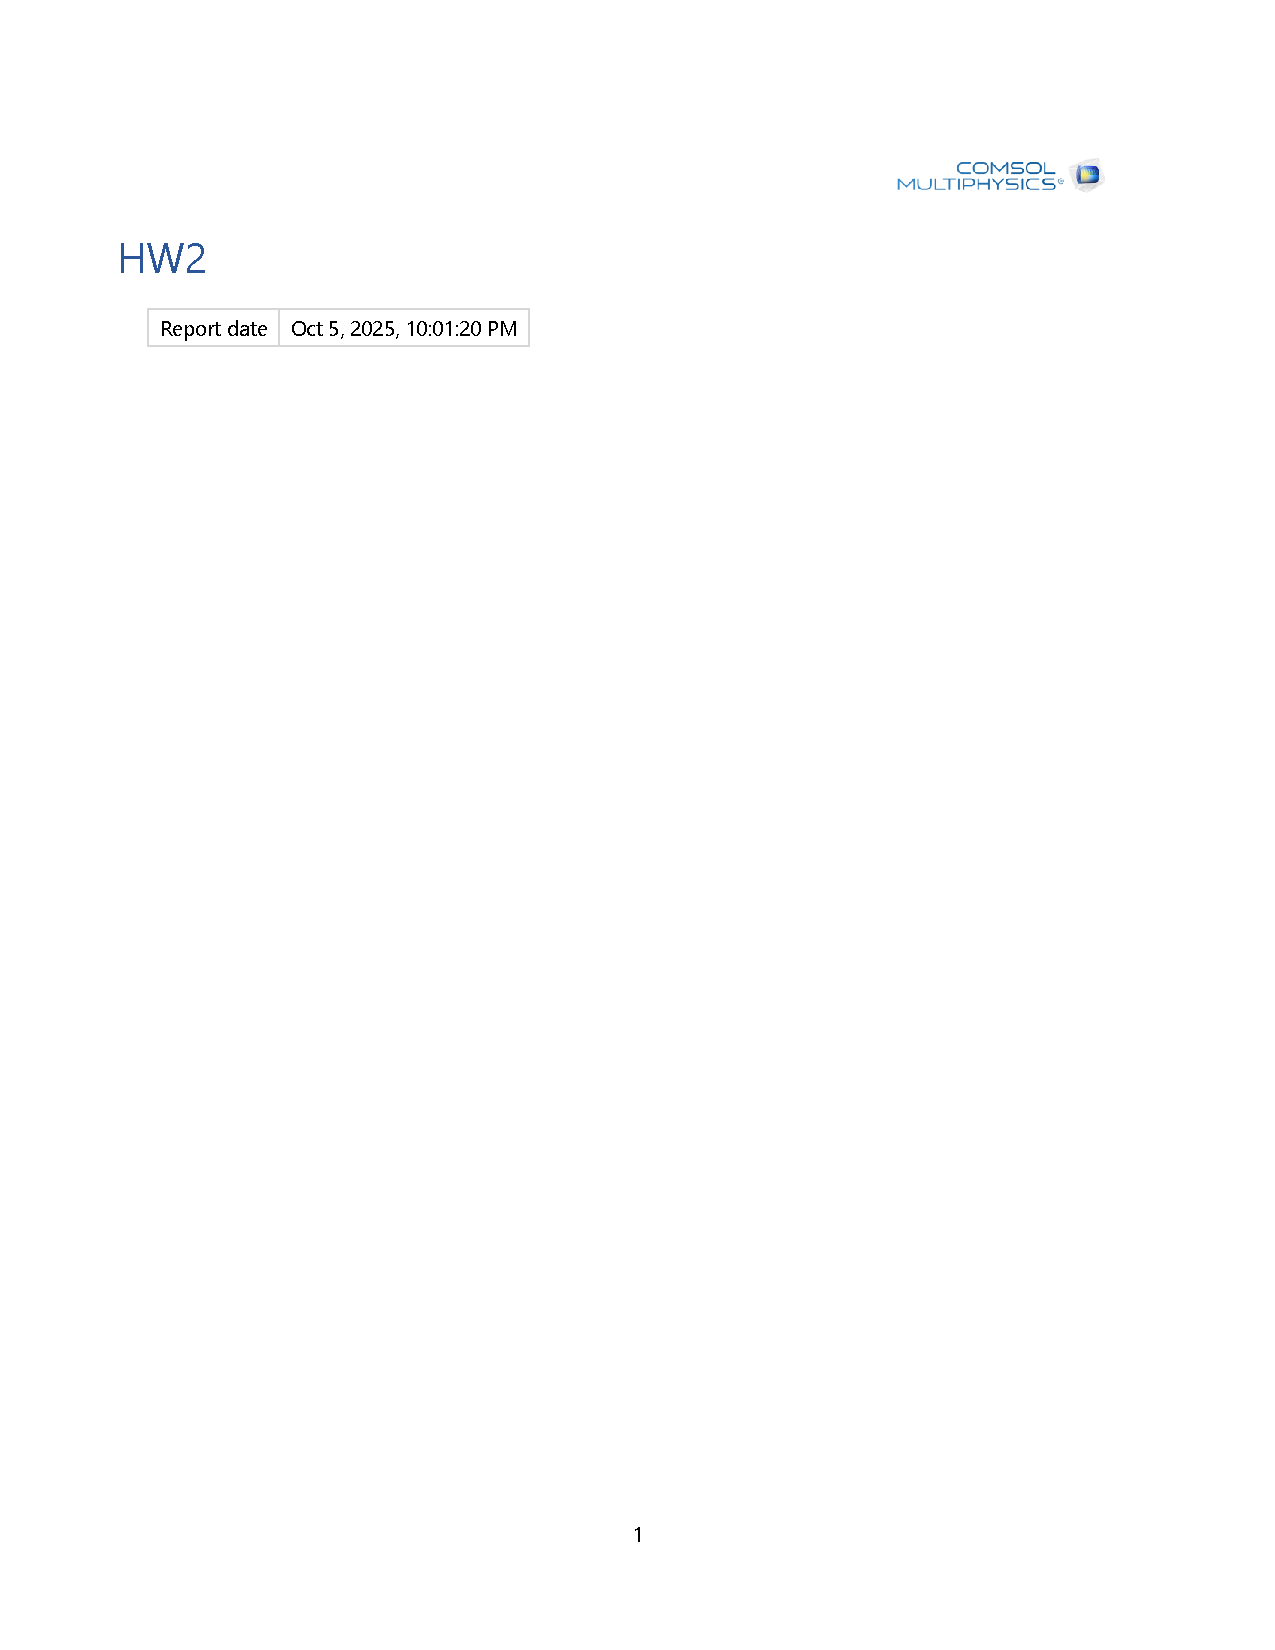
\includepdf[pages=-]{HW2comsol.pdf}

\end{document}